\documentclass[12pt,letterpaper,boxed]{hmcpset}
\usepackage[margin=1in,headheight=14pt]{geometry}
\usepackage{amsfonts, amsmath, amssymb, enumerate, fancyhdr, gensymb, lastpage, mathtools, parskip, graphicx}
\usepackage{xcolor, tikz-cd}
\newcommand{\wg}[1]{\textcolor{violet}{#1}}
\newcommand{\OO}{\mathcal O}
\newcommand{\Q}{\mathbb Q}
\newcommand{\R}{\mathbb R}
\newcommand{\C}{\mathbb C}
\newcommand{\Z}{\mathbb Z}
\newcommand{\abs}[1]{\left|#1\right|}
\newcommand{\im}{\text{im }}
\newcommand{\inv}{^{-1}}
\newcommand{\normal}{\unlhd} %% one can also use \trianglelelefteq
\newcommand{\anglee}[1]{\langle #1 \rangle}
\usepackage[shortlabels]{enumitem}
\newenvironment{wgenv}{\color{violet}}{}

% Numbering macros
\pagestyle{fancy}
\lhead{Will Gilroy}
\chead{Complex Homework \#8}
\rhead{25 March 2026}
\lfoot{}
\cfoot{}
\rfoot{Page\ \thepage\ of\ \pageref{LastPage}}

\linespread{1.5}

\newcommand\blankpage{
    \thispagestyle{empty}
    \addtocounter{page}{-1}
    \newpage}
\renewcommand\footrulewidth{0.4pt}

\begin{document}

\problemlist{Complex Analysis Homework \#8} 

%------------------------- Problem 1 -----------------------

\begin{problem}
	
\includegraphics[scale=0.8]{1.png}
	\hfill
\end{problem}

\begin{solution}
If a function $\hat \C \to \hat \C$ is holomorphic then it restricts
to a holomorphic function $\C \to \C$, since $\C$ is open in
$\hat \C$. So we first consider
holomorphic functions $\C \to \C$ and then understand how they can be 
extended to $\hat \C$.
Recall the holomorphic functions $\C \to \C$. 
These are exactly functions with a single power series representation
\[
	f(z) = c_0 + c_1z + c_2z^2 + \cdots,
\]
with infinite radius of convergence (i.e. such that $\limsup
\abs{c_n}^{1/n} = 0$).

To extend a holomorphic function $f: \C \to \C$ to a function on $\hat
\C$ we must only specify its value at $\infty$. To verify that it's a
holomorphic extension we must then check that our extended function is
holomorphic at $\infty$.

If $f: \C \to \C$ holomorphic is constant $f(z) = k$ then, by continuity, we must
have that $f(\infty) = k$. In this case, $f: \hat \C \to \hat \C$ is
holomorphic since the extended function is a constant function on
$\hat \C$. 
On the other hand, if $f$ is non-constant then it must be unbounded.
I.e. $\lim_{\abs{z} \to \infty} f(z)$ converges for all approaches and takes value
$\infty$.
And so, again, by continuity we must have $f(\infty) = \infty$.
To make sense of this last statement we can view our extended $f$ ``in
the other patch'' given by the transition $z \mapsto 1/z$. In this
sense, we can view $f(\infty)$ as $f(1/z)$, and we have defined this
value to be $0$ as $z \to 0$.
\wg{We have argued how to continuously extend a non-constant
holomorphic function from $\C$ to $\hat \C$, but we need to argue that
this extension is holomorphic at $z = \infty$. }

\end{solution}

\newpage

%------------------------- Problem 2 -----------------------

\begin{problem}
	
\includegraphics[scale=0.8]{2.png}
	\hfill
\end{problem}

\begin{solution}
First recall that the argument principle states, given a holomorphic
function $f: U \to \C$, an open set $V \subseteq U$ with $\bar V
\subseteq U$ and $f$ nonvanishing on $\partial V$, we have 
\[
	\int_{\partial V} \frac{f'(z)}{f(z)} dz = 2\pi i \sum_{p \in V} Mult_p(f).
\]
In particular, it is sufficient to show then that there is an $n$
large enough so that $\int_{\partial D(0,R)} (f_n)'/f_n dz = 0$. 

First notice that 
\[
	(f_n)'(z) = 1 + z + \frac{z^2}{2!} + \cdots + \frac{z^{n-1}}{(n-1)!}.
\]
And so 
\[
	\frac{f'(z)}{f(z)} = 1 - \frac{z^n}{n!} \frac{1}{f(z)}.
\]
Then
\begin{align*}
	\int_{\partial D} \frac{f'}{f} dz
	&= \int_{\partial D} 1 - \frac{1}{n!}\frac{z^n}{f(z)}dz \\
	&= -\frac{1}{n!} \int_{\partial D} \frac{z^n}{f(z)} dz.
\end{align*}
By Cauchy's integral theorem, since $f(z) = 1$ is entire. And now, we can understand this remaning
integral in terms of the residue theorem 
\[
	\int_{\partial D} \frac{z^n}{f(z)}dz = 2\pi i \sum_{p \in D} res_p(z^n/f_n(z)).
\]
It is only possible for us to have a non-zero residue at a point $p$
if $f_n(p) = 0$. And so, let us consider where the zeroes of $f_n(z)$
may lie. In particular, if there exists an $n$ such that all the
zeroes of $f_n(z)$ lie outside of $D(0,R)$ then we have shown what we
have set out to show.

\wg{I wasn't totally sure how to bound the magnitude of the zeroes
from here. One thing I thought of doing was attempting to consider
$f_n(z) = e^z - \sum_{k=n}^{\infty} z^k/k!$ and so $f_n(z) = 0$
if and only if $e^z = \sum_{k=n}^\infty z^k/ k!$. I could attempt to
apply log to both sides and then poke at the symbols. }


\wg{Here's another idea that I thought about.}
Suppose that for all $n$ there existed some $z_0$ a zero of $f_n$ with $\abs{z_0}
\leq R$ for all $n$. Since the series $\lim_{n \to \infty} f_n(z) =
e^z$ converges uniformally, I wonder if this might imply that $e^z$
has a zero in $\C$ (which would be a contradiction). But I'm not sure
I have a theorem that says anything like this at hand.

\end{solution}

\newpage

%------------------------- Problem 3 -----------------------

\begin{problem}
	
\includegraphics[scale=0.8]{3.png}
	\hfill
\end{problem}
\begin{solution}
First I claim that the number of fixed points of a Mobius
transformation is an invariant of its conjugacy class.
Suppose a Mobius transformation is represented by $A \in PGL_2(\C)$
and suppose it fixed a vector $v$. Then a conjugation $B A B\inv$ for
some $B \in PGL_2(\C)$ 
is tantamount to a change of basis of $A$. In particular 
$(BA B\inv) (Bv) = Bv$ and so $BA B\inv$ fixes $Bv$ --- a fixed vector
of $A$ maps to a fixed vector of any of its conjugates. 
Moreover, this process is inverted by 
conjugating again $B\inv (B A B\inv) B = A$. And so, since Mobius
transformations are in particular bijections, the number of fixed
points is a well-defined invariant of its conjugacy class.

We consider the possible number of fixed points of a Mobius transformation.
By triple transitivity we know that there's a unique Mobius
transformation which sends one triple of distinct points to another
triple of distinct points. And so if a Mobius
transformations fixes at least three points, it must be the identity.
Hence, a non-identity Mobius transformation must fix either $0,1,2$
points. \wg{Neither of these transformations appear to fix zero
points. Note, by inspecting the equation $f(z) = z$ for a general
Mobius transformation, I think we can show that there's no Mobius
transformation which fixes zero points.}

Now consider the given functions. Note that $\lambda z = z$ is solved
only by $z= 0$ if $\lambda = 1$. If $\lambda = 1$ then $f(z) =
\lambda z$ is the identity map. In both cases $f(z) = \lambda z$ also
fixes the point at infinity.
Likewise $z + 1 = z$ is not solved for $z \in \C$, however, the
point at infinity is fixed by this map.
Hence the maps $f(z) = \lambda z$ and $f(z) = z +1$ have two fixed
points and one fixed point respectively. 

We have argued that the number of fixed points is well-defined
invariant of the conjugacy classes of $PGL_2(\C)$, and that a
non-identity Mobius transformation can only have $0,1$, or $2$ fixed
points.
But we also need to
argue that there are only three conjugacy classes in $PGL_2(\C)$.
That is, a priori there could be multiple conjugacy classes of $PGL_2(\C)$
with a given number of fixed points.

\wg{Apologies, the following will be a bit rambly. I was hoping 
to characterize the Mobius transformations based on the solutions to 
the equation $f(z) = z$.}
Let $f(z) = (az + b)/(cz+d)$ be a Mobius transformation. Note that 
$f(z) = z$ is given by the quadratic equation 
\[
	cz^2 + (d-a)z - b = 0.
\]
First suppose that $c = 0$, then this equation has two distinct
solutions in $z$ if $(d-a)^2 + 4bc \neq 0$. Otherwise it has at least
one solution.

In the case where $c = 0$ our fixed point equation becomes 
\[
	(d-a)z -b = 0.
\]
If $d=a$ then our Mobius transformation is equivalent to $f(z) = (z +
\tilde b)/1$ which only has a fixed point at infinity. Likewise if $d
\neq a$ then we have a fixed point $z = b/(d-a)$ but also our Mobius
transformation is equivalent to $f(z) = \tilde a z - \tilde b$. 

Without loss of generality, we can choose our coordinate system so
that one fixed point is at $\infty$. For $\infty$ to be fixed we must
have $c=0$ \wg{I am guessing here, I suppose this needs to be shown
better.} 
Then the fixed point equation $f(z) = z$ becomes $(a-d)z = -b$. 
\wg{From this point I would try to explicitly construct the change 
of basis matrices which sends $f$ to $\lambda z$ if $a \neq d$ (I
suppose this is the transformation which further sends $-b/(a-d)$ to
$0$), and the change of basis which sends $f$ to $f + 1$ if $a = d$. }
\end{solution}

\newpage

%------------------------- Problem 4 -----------------------

\begin{problem}
	
\includegraphics[scale=0.8]{4.png}
	\hfill
\end{problem}

\begin{solution}
First note that it is sufficient to find $g \in \C(x)$ such that
$g^{\circ 3} = z + 1$ or $g^{\circ 3} = \lambda z$ for $\lambda \neq
0$.
If $g^{\circ 3} = h f h\inv \in PGL_2(\C)$ then notice 
\[
	(h\inv g h)^{\circ 3} = h\inv g^{\circ 3} h 
		= h\inv (h f h\inv) h	
		= f.
\]
That is, if we find a rational $g$ with $g^{\circ 3}$ in some
conjugacy class of a mobius transformation, then we have found the $g$
such that $g^{\circ 3} = f$ for all $f$ in the same conjugacy class.

Consider first $g$ as a degree $1$ rational function.
Note that we can represent degree $1$ rational functions as matrices with the
same method that we have been representing mobius transformations as
matrices (except now the representation of some rational functions
will have zero determinant). And so we can use matrix multiplication
to compute the compositions a bit more easily.

Consider first $f(z) = \lambda z$. Consider rational functions of the
form 
\[
	[g]^3 = \begin{bmatrix}
		\alpha & 0 \\ 0 & 1
	\end{bmatrix}^3 
	= \begin{bmatrix}
		\alpha^3 & 0 \\ 0 & 1
	\end{bmatrix}. 
\]
And so we will have $g^3 =f$ for each solution of $\alpha^3 - \lambda
= 0$ in $\C$. But recall that $\C$ is algebraically closed and so for
a fixed $\lambda$ we have three solutions to this equation. 
The discriminant to this cubic equation is $\Delta =
\lambda(-27\lambda + 18)$ is not zero unless $\lambda = 18/27$. 
And so for most $\lambda$ we have three distinct solutions to this
equation.
And so, we have at
least three solutions to $g^3(z) = \lambda z$.
\wg{could there be any other solution?}

\wg{how about for the other function?}
\begin{wgenv}
	For $f(z) = z + 1$ we have that 
	\[
	\begin{bmatrix}
		1 & 1/3 \\ 0 & 1
	\end{bmatrix}^3 =
	\begin{bmatrix}
		1 & 1 \\ 0 & 1
	\end{bmatrix}.
	\]
	However we haven't said anything about whether 
	any other degree $1$ map might cube to give the desired map.
	In particular, I think it is possible for a power of a non-upper triangular
	matrix to become upper triangular.

	Lastly, we would need to address non-degree $1$ rational functions.
\end{wgenv}

\end{solution}


\newpage

%------------------------- Problem 5 -----------------------

\begin{problem}
	
\includegraphics[scale=0.8]{5.png}
	\hfill
\end{problem}

\begin{solution}
First consider the following plot of $Re(e^{1/z})$ from desmos.

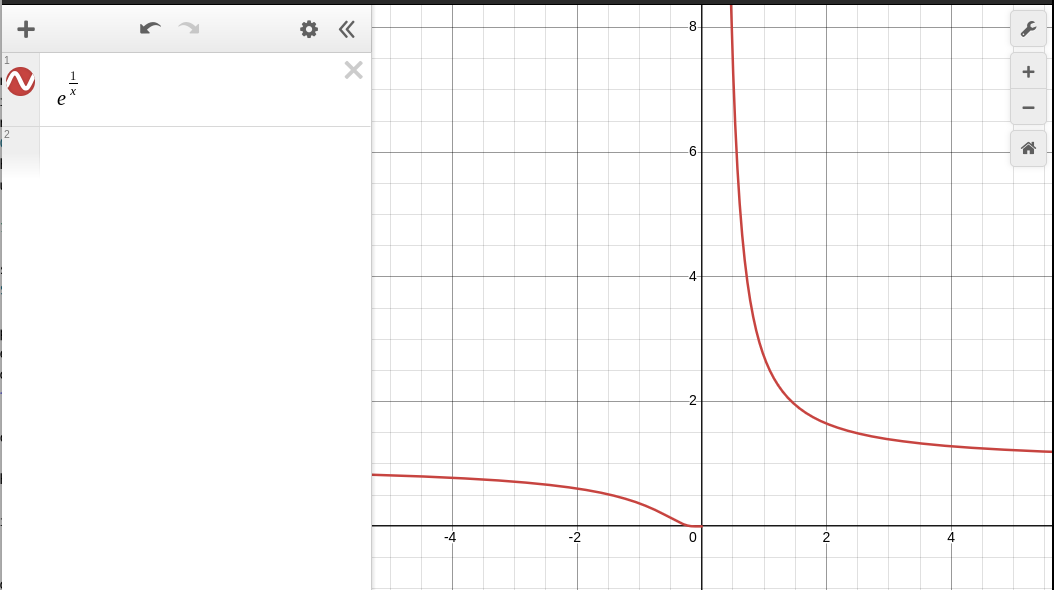
\includegraphics[scale=0.6]{desmos-memes.png}

This plot suggests that a sequence approaching $0$ along the negative
real axis may give us what we want. 
Let $z_n = -1/n \in \R$. We have that $z_n \to 0$. 
First notice that
\[
	\lim_{n \to \infty} 1/z_n = \lim_{n \to \infty} -n ``='' -\infty
\]
And we so we have
\[
	\lim_{n \to \infty} e^{1/z_n} 
	= \lim_{u \to -\infty} e^{u}
	= 0.
\]



\end{solution}

\newpage

%------------------------- Problem 6 -----------------------

\begin{problem}
	
\includegraphics[scale=0.8]{6.png}
\end{problem}

\begin{solution}
To begin, suppose that the zeroes of $f(z)$ are $z_1, \cdots, z_n \in
\Delta$. 
Then, I claim that we can write $f(z) = (z- z_1) \cdots (z - z_n)
g(z)$ where $g$ is a non-vanishing holomorphic function on $\Delta$.

Recall that, by inspecting the power series of $f$ about a zero, say
$z_1$, we can write $f(z) = (z-z_1) g_1(z)$ locally about $z_1$ for some $m$ and where
$g_1$ is non-vanishing on a neighbourhood of $z_1$ (since the zeroes
are isolated). 
But now $g_1$ is a holomorphic function on $\Delta$ with zeroes at the
remaning points $z_2, \cdots, z_n$. And so, about $z_2$ we can write
$g_1(z) = (z-z_2)g_2(z)$ where $g_2$ is non-vanishing on a
neighbourhood of $z_2$. Note that $g_2$ is also non-vanishing on a
neighbourhood of $z_1$ because $g_1$ is.
Now, we can write $f(z) = (z-z_1)(z-z_2)g_2(z)$. Continuing this
process yields the claimed form of $f$.
Note that this construction deals with $n$ distinct zeroes of $f$ in
$\Delta$, however, essentially the same construction can be used if we
have ``repeated zeroes'' (unclear to me whether that's disallowed in the
question set-up). 

Now applying the product rule to compute $f'(z)$ yields
\[
	f'(z) = \sum_{i=1}^n (\Pi_{k \in ([n]\setminus i)} (z-z_i) g(z)) + \Pi_{i=1}^n (z-z_i) g'(z)
\]
And then 
\[
	\frac{f'(z)}{f(z)} = \sum_{i=1}^n \frac{1}{z-z_i} + \frac{g'(z)}{g(z)}
\]

Recall that the argument principle will yield
\[
	\frac{1}{2\pi i} \int_{S^1} \frac{f''(z)}{f'(z)} = \sum_{p \in \Delta} Mult_p(f')
\]
So long as $f'(z)$ does not vanish on $S^1$. 

\begin{wgenv}
Now, if there were some relationship between $f''/f'$ and $f'/f$ 
I could rewrite the desired integral in terms of the things that we
know. I think there might be something like this. 
Recalling that $f''/f'$ is called the ``logarithmic derivative of
$f'$'' we could notice that 
\[
	f''/f' = \frac{d}{dz} \log(f') = \frac{d}{dz} \log(f'/f \cdot f)
	= \frac{d}{dz} \log(f'/f) + f'/f,
\]
However, applying something like this to the desired integral is not
super clear to me. 
On the other
hand the $f'/f$ term contains the term $g'(z)/g(z)$, the integral of
which should come to $0$ since $g$ is nonvanishing on $\Delta$. 

Moreover, the question is asking ``prove or disprove''. And so, I
could have attempted this question by inspecting particlar holomorphic functions on
the unit disc, and attempted to inspect their derivatives. 
\end{wgenv}

\end{solution}

\newpage



\end{document}
